\documentclass[conference]{IEEEtran}
\IEEEoverridecommandlockouts

\usepackage{cite}
\usepackage{amsmath,amssymb,amsfonts}
\usepackage{graphicx}
\usepackage{textcomp}
\usepackage{xcolor}

\usepackage{subcaption}

\usepackage{tikz}
\usepackage{pgfplots}

\usepackage{cleveref}
\usepackage{csquotes}
\usepackage{booktabs}

\usepackage{flushend}

\usetikzlibrary{patterns}

\definecolor{tol1}{HTML}{33bbee}
\definecolor{tol2}{HTML}{009988}
\definecolor{tol3}{HTML}{ee7733}
\definecolor{tol4}{HTML}{cc3311}
\definecolor{tol5}{HTML}{66CCEE}
\definecolor{tol6}{HTML}{CD7F32}

\definecolor{plt1}{HTML}{4053d3}
\definecolor{plt2}{HTML}{ddb310}
\definecolor{plt3}{HTML}{b51d14}
\definecolor{plt4}{HTML}{00beff}
\definecolor{plt5}{HTML}{fb49b0}

\pgfplotscreateplotcyclelist{bwb}{%
  thick, tol1\\%
  thick, tol2\\%
  thick, tol3\\%
  thick, tol4\\%
  thick, tol5\\%
  thick, tol6\\%
}

\usepackage{acro}
\DeclareAcronym{cots}{
  short = COTS,
  long = off-the-shelf,
}

\newcommand\MP{\ensuremath{\mathrm{MP}}\xspace}
\newcommand\SNR{\ensuremath{\mathrm{SNR}}\xspace}

\newcommand\ours{\textsc{JscCaF}\xspace}

\DeclareAcronym{tiff}{
  short = TIFF,
  long = tag image file format,
}

\DeclareAcronym{mse}{
  short = MSE,
  long = mean squared error,
}

\DeclareAcronym{awgn}{
  short = AWGN,
  long = additive white Gaussian noise,
}

\DeclareAcronym{pdf}{
  short = PDF,
  long = probability-density function
}

\DeclareAcronym{leo}{
  short = LEO,
  long = low Earth orbit,
}

\DeclareAcronym{ldpc}{
  short = LDPC,
  long = low-density parity-check,
}

\DeclareAcronym{jscc}{
  short = JSCC,
  long = joint source and channel coding,
}

\DeclareAcronym{djscc}{
  short = DJSCC,
  long = deep joint source and channel coding,
}

\DeclareAcronym{snr}{
  short = SNR,
  long = signal-to-noise ratio,
}

\DeclareAcronym{cnn}{
  short = CNN,
  long = convolutional neural network,
}

\DeclareAcronym{psnr}{
  short = PSNR,
  long = peak signal-to-noise ratio,
}

\DeclareAcronym{prelu}{
  short = PReLU,
  long = parameterized rectified linear unit,
}

\DeclareAcronym{relu}{
  short = ReLU,
  long = rectified linear unit,
}

\DeclareAcronym{jscc-sat}{
  short = \textsc{JSCC-Sat},
  long = {joint source-and-channel coding for small satellite applications}
}

\DeclareAcronym{los}{
  short = {LOS},
  long = {line of sight}
}

\DeclareAcronym{esa}{
  short=ESA,
  long=European Space Agency
}

\usepackage{xspace}
\newcommand\cubesat{CubeSat\xspace}
\newcommand\cubesats{\cubesat{}s\xspace}

\newcommand\jpegtwok{JPEG\,2000\xspace}

\newcommand\sentinelii{Sentinel-2\xspace}

\begin{document}

\title{Adaptable Joint Source-and-Channel Coding for Small Satellite Applications}

\author{\emph{Anonymous authors}}
% \author{\IEEEauthorblockN{Olga Kondrateva}
% \IEEEauthorblockA{\textit{Humboldt-Universit\"at zu Berlin}\\
% Berlin, Germany \\
% kondrate@informatik.hu-berlin.de}
% \and
% \IEEEauthorblockN{Stefan Dietzel}
% \IEEEauthorblockA{\textit{Merantix Momentum GmbH}\\
% Berlin, Germany \\
% stefan@merantix-momentum.com}
% \and
% \IEEEauthorblockN{Bj\"orn Scheuermann}
% \IEEEauthorblockA{\textit{Technical University of Darmstadt}\\
% Darmstadt, Germany \\
% scheuermann@kom.tu-darmstadt.de}
% }

\maketitle

\begin{abstract}
Earth observation using small satellites serves a wide range of relevant applications.
However, significant advances in sensor technology (e.g., higher resolution, multiple spectrums beyond visible light) in combination with challenging channel characteristics lead to a communication bottleneck 
when transmitting the collected data to Earth.
Recently, joint source coding, channel coding, and modulation using a neuronal-network-based approach has been proposed to combine image compression and communication. %dynamically adapt to the varying communication channel and to take data properties into account.
Though this approach achieves promising results when applied to standard terrestrial channel models, 
it remains an open question whether it is suitable for the more complicated and quickly varying satellite communication channel. 
In this paper, we consider a detailed satellite channel model accounting for different shadowing conditions and train an encoder-decoder architecture using realistic \sentinelii satellite imagery.
In addition, to reduce the overhead associated with using multiple neural networks for various channel states, 
we leverage attention modules and train a single adaptable neural network that covers a wide range of different channel conditions.
Our evaluation results show that the proposed approach achieves on-par performance when compared to less space efficient schemes using separate neuronal networks for differing channel conditions.   
% it typically involves training multiple neural networks to account for different channel conditions  
% In this paper, we propose a novel joint coding scheme that combines image compression, channel coding, and modulation using a neuronal-network-based approach.
% By combining a detailed channel model for small satellite applications with attention modules, we can use a single adaptable neuronal network to cover a wide range of different channel conditions.
% We evaluate our approach using realistic \sentinelii satellite imagery and show that it achieves on par performance when compared to less space efficient schemes using separate neuronal networks for differing channel conditions.
\end{abstract}

\begin{IEEEkeywords}
  cross-layer optimization; AI-enabled networking; small satellite applications
  \end{IEEEkeywords}

\acresetall
\section{Introduction}

Earth observation using sensor data acquired by satellites has gained more and more attention over the last years.
Common use cases include environment monitoring \cite{rs14030589}, disaster management \cite{barmpoutis2020}, and many more \cite{radix,MarCO}.
The increasing momentum can be explained by two major factors.
First, technological advances have allowed to build smaller satellite classes, which use more off-the-shelf components and can be deployed more easily.
A prime example are CubeSats, which operate in \ac{leo} and consist of $10 \times 10 \times 10$\,cm units \cite{cubesat2020}.
Second, sensor technology has improved greatly.
Besides higher resolution, modern sensors support a wider spectrum range, exceeding that of visible light.
Hyper-spectral images include infrared and other bands, which can be used monitor vegetation, clouds, and other phenomena not represented in the visible light spectrum.

These advances in satellite and sensor technology, however, are not met by an equal improvement in communication capacity.
CubeSats and other small satellites have a constrained energy budget, and -- unlike their larger counterparts -- they are not geo-stationary.
That is, they orbit the Earth several times per day with high speed, limiting communication with ground stations to several short communication windows.
Their high velocity and interferences due to harsh weather and potential non line-of-sight conditions further lead to high packet loss rates and complicate communication \cite{nogales2018}.

Therefore, efficient and robust coding schemes are a necessity to support demanding Earth observation applications.
Typically, source coding, channel coding, and modulation schemes are combined to translate image sensor data into physical layer channel symbols.
Source coding serves to compress sensor images, often using lossy compression schemes, such as \jpegtwok \cite{sentinel-2-user-handbook}.
Channel coding (e.g., \ac{ldpc}) is then used to enable error correction, counteracting packet loss due to the harsh channel conditions.
More recently, approaches that consider these coding mechanisms jointly have emerged, promising better than performance than using individual coding schemes \cite{6408177}.
Joint coding leverages the data-centric nature of the considered use case: the characteristics of the hyper-spectral image sensor data is well known, and therefore, the image data can be translated directly into physical layer symbols rather than using separate source codes, channel codes, and modulation.
And although Shannon's theory \cite{cover1991elements} states that separate optimization should yield optimal results, this is not true in practice due to hypothetical assumptions, such as infinite code block lengths.

The use of neuronal networks has provided a feasible way to implement such a joint coding approach, improving over earlier work, which was too complex to be useful in practice \cite{9838671}.
Neuronal-network-based joint coding approaches have been proposed for both terrestrial communication \cite{Bourtsoulatze2019} and satellite applications \cite{satjscc}.
So far, a major limitation has been that the joint encoder and decoder has been trained based on fixed assumptions about channel characteristics, such as the \ac{snr} using a simple \ac{awgn} channel model.
To accommodate changing channel conditions, separate neuronal networks need to be trained independently and switched between by both the satellite and the ground station.
Obviously, this approach restricts the total number of channel parameter combinations that can reasonably be covered.
Considering more complex channel models including multi-path propagation, shadowing, and fading would easily lead to a combinatorial explosion of parameters, and consequently a prohibitive amount of separate neuronal networks.

In this paper, we propose a novel joint coding approach for satellite applications that allows to use a single neuronal network for a wide range of channel conditions typical for small satellite applications.
We use a neuronal network model architecture that is enriched by so-called attention modules to reduce the combinatorial complexity.
Using this architecture, we can train a single neuronal network based on a number of different channel conditions.
During operation, the attention modules allow to essentially parametrize the network for different actual channel conditions.
This parametrization allows us to consider a wide range of realistic channel conditions for small satellite applications.
To model the channel, we use Fontán et al.'s channel model \cite{fontan2001}, which is applicable to non-geostationary small satellites and models a number of channel characteristics, such as multi-path propagation and shadowing.
More specifically, we consider three scenarios -- \ac{los}, shadowing, and deep shadowing -- to capture different extents of multi-path propagation and shadowing effects.
In addition, we also consider different levels of \ac{snr} to model satellite elevation angles and other parameters.
During training of the encoder-decoder neuronal network, these parameters are used as input, in addition to a large number of example satellite images.
Whereas a traditional encoder-decoder network would then -- simply speaking -- learn a coding scheme for the \enquote{average} of all parameters, the attention modules allow to embed schemes for all parameters within a single network that can be dynamically parameterized with the actual channel conditions during use.
Therefore, a single network suffices when using attention modules, and separate networks with a simpler architecture are required in order to precisely represent different channel conditions.
Although the resulting network with attention modules is larger than one trained for a specific set of channel conditions, it is considerably smaller than considering a set of separate networks, one for each channel condition.

Our evaluation using a set of hyper-spectral images from the \sentinelii mission shows that our approach performs as good as separate, individual networks for different channel conditions while requiring significantly lower storage overhead.

Thus, our main contributions can be summarized as follows:
%
\begin{enumerate}
  \item We combine \ac{jscc} approaches with a realistic channel model for small satellite applications.
  \item We apply an attention-module-augmented neuronal network architecture to be able to use a single network for a wide range of realistic channel characteristics.
  \item We evaluate our approach using a set of realistic \sentinelii Earth observation data.
\end{enumerate}

The remainder of this paper is organized as follows.
In \Cref{sec:related_work}, we review existing work on \ac{jscc}, source coding, channel models, and attention modules.
Next, we provide an overview of our system model in \Cref{sec:system_model} before explaining our mechanism in detail in \Cref{sec:our_approach}.
\Cref{sec:evaluation} details our evaluation results using \sentinelii mission data.
We conclude the paper in \Cref{sec:conclusion}.

\section{Related Work}
\label{sec:related_work}

\begin{itemize}
  \item LCN23
  \item Channel models for satellites
  \item Attention modules
\end{itemize}



\section{Earth Observation Missions}
\label{sec:system_model}

\begin{figure*}
  \begin{subfigure}{.32\linewidth}
    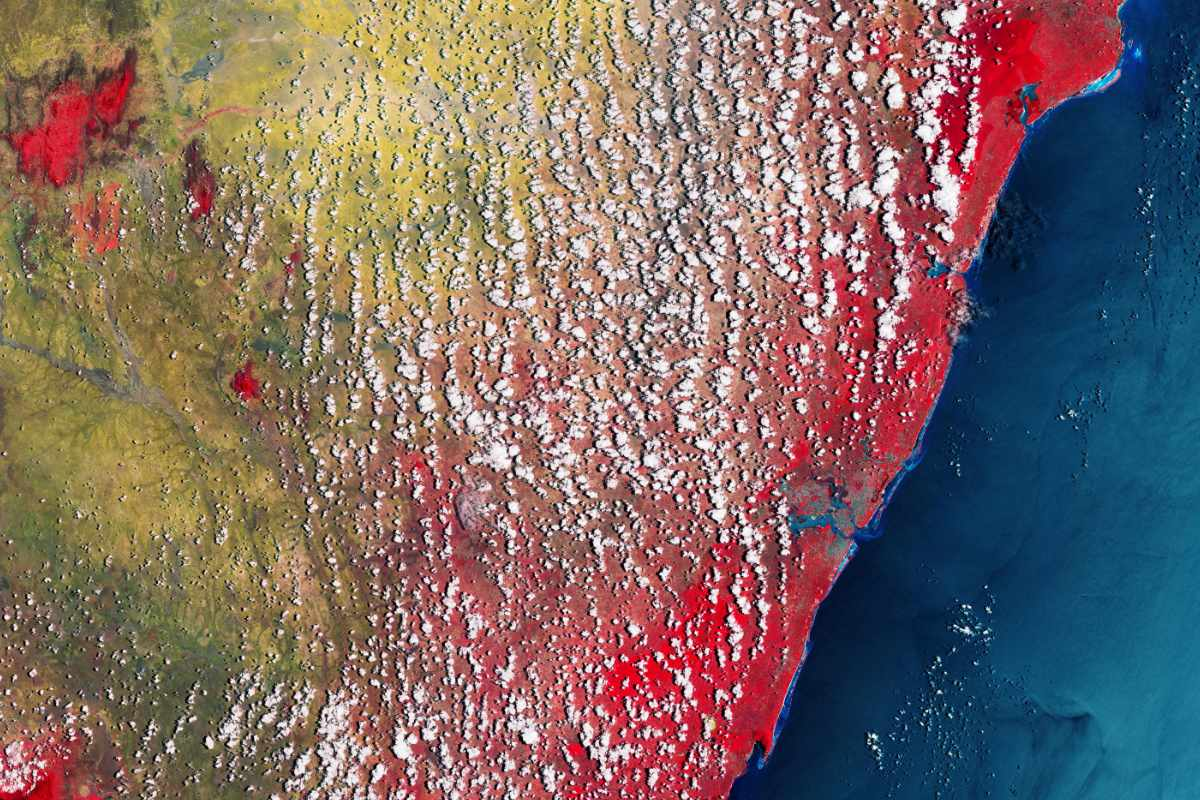
\includegraphics[width=\linewidth]{figures/Earth_from_Space_Southeast_Kenya}
    \caption{Southeast Kenya}
    \label{fig:sentinel_kenya}
  \end{subfigure}
  \hfill
  \begin{subfigure}{.32\linewidth}
    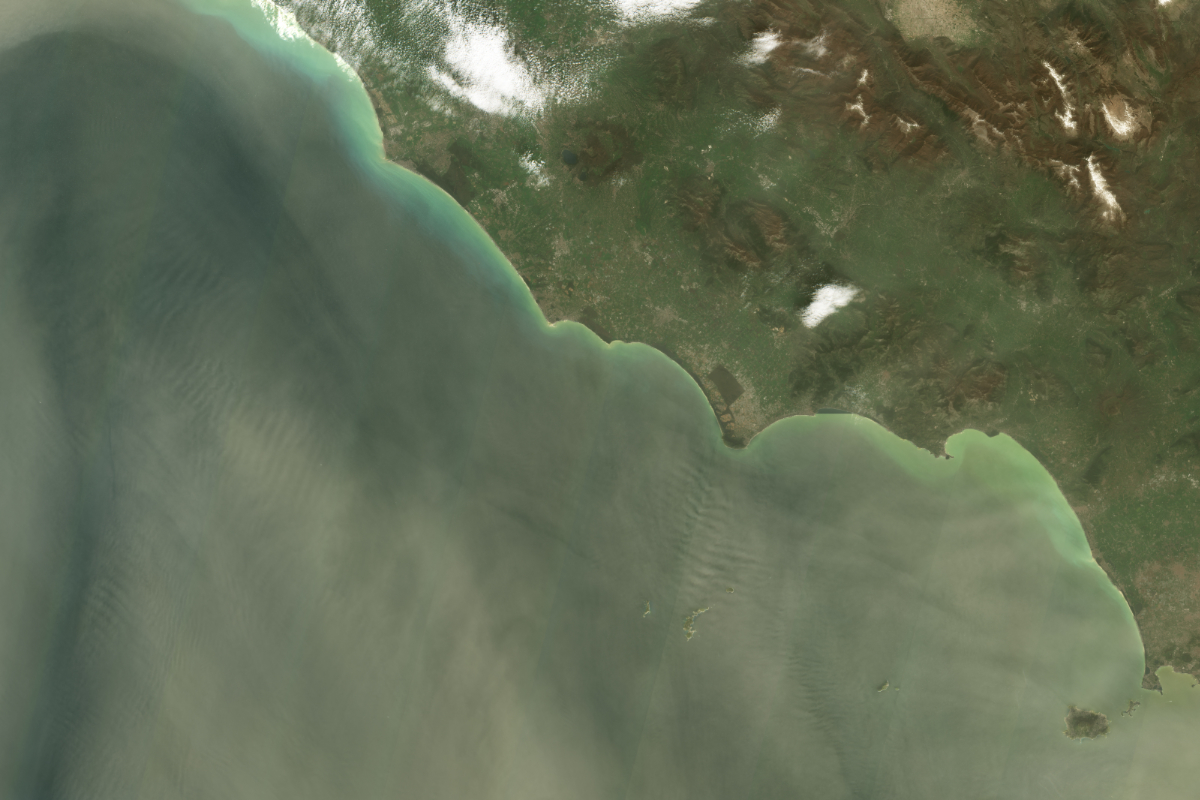
\includegraphics[width=\linewidth]{figures/Saharan_dust_plume}
    \caption{Sahara dust}
    \label{fig:sentinel_sahara}
  \end{subfigure}
  \hfill
  \begin{subfigure}{.32\linewidth}
    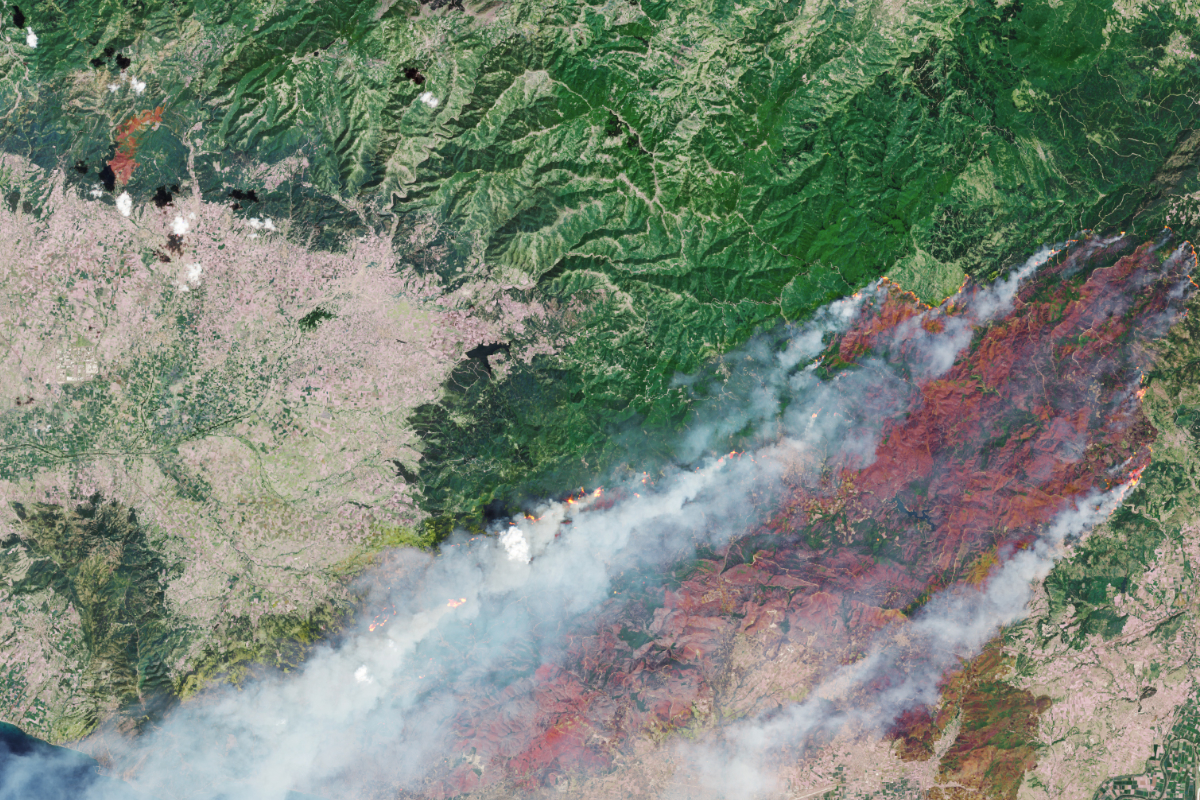
\includegraphics[width=\linewidth]{figures/Wildfires_continue_to_rage_in_Greece}
    \caption{Wildfires in Greece}
    \label{fig:sentinel_greece}
  \end{subfigure}

  \caption{Example images from the \sentinelii mission. (Credit: processed by ESA, CC BY-SA 3.0 IGO)}
  \label{fig:sentinelii}
\end{figure*}

\begin{table}
  \caption{\sentinelii Spectrum Bands}
  \label{tab:sentinel_bands}

  \centering
  \begin{tabular}{llcc}
    \toprule
    Band & Measurement & Central wavelength & Resolution \\
    \midrule
    1 & Coastal aerosol & 443 nm & 60 m \\
    2 & Blue & 490 nm & 10 m \\
    3 & Green & 560 nm & 10 m \\
    4 & Red & 665 nm & 10 m \\
    5 & Vegetation red edge & 705 nm & 20 m \\
    6 & Vegetation red edge & 740 nm & 20 m \\
    7 & Vegetation red edge & 783 nm & 20 m \\
    8 & Near infrared & 842 nm & 10 m \\
    8A & Narrow near infrared & 865 nm & 20 m \\
    9 & Water vapour & 940 nm & 60 m \\
    10 & Short wave infrared: cirrus & 1375 nm & 60 m \\
    11 & Short wave infrared & 1610 nm & 20 m \\
    12 & Short wave infrared & 2190 nm & 20 m \\
    \bottomrule
  \end{tabular}
  
\end{table}

With recent advances in space and image sensing technologies, Earth observation using small satellites has gained more and more attention over the past years.
As an example use case for the methods we propose in this paper, we briefly introduce ESA's \sentinelii mission.
We also use a subset of the mission's dataset for our evaluation.
Moreover, we give an overview of how neuronal networks are used onboard satellites for image processing.

\sentinelii \cite{sentinel2} is a set of missions operated by the \ac{esa} as part of the Copernicus program using \ac{leo} satellites.
The first satellites were launched in 2015, with more launches following in 2017 and 2024.
The missions comprise two satellites, which orbit the Earth such that each spot on the surface is revisited approximately every five days.
With their sensors, they cover a strip of land that is 290 km wide with each pass.
In addition to visible light sensors, the satellites are equipped with sensors that cover additional frequencies, such as infrared \cite{sentinel-2-user-handbook}, which allow to capture land use and vegetation (cf. \Cref{tab:sentinel_bands}).
Moreover, the sensors feature relatively high optical resolutions between 10 and 60 meters.

% https://www.esa.int/ESA_Multimedia/Images/2024/03/Earth_from_Space_Southeast_Kenya
% https://www.esa.int/ESA_Multimedia/Images/2024/04/Saharan_dust_plume
% https://www.esa.int/ESA_Multimedia/Images/2023/08/Wildfires_continue_to_rage_in_Greece

\Cref{fig:sentinelii} shows three example use cases for Earth observation images taken from \ac{esa}'s homepage.
The first (\Cref{fig:sentinel_kenya}) is a false-color image of southeast Kenya, which was generated by overlaying \sentinelii's near-infrared channel onto the visual spectrum.
The bright red colors indicate higher plant density and health, as alive plants reflect near-infrared light.
Thereby, the dense vegetation in the coastal regions can easily be distinguished from the hinterland regions.
\Cref{fig:sentinel_sahara} shows a dust storm originating from the Sahara desert.
\sentinelii provides valuable insights for air pollution monitoring, and due to the short revisit time, storms can be monitored as they develop.
Finally, \Cref{fig:sentinel_greece} shows wildfires in Greece in 2023.
For the visualization, the shortwave infrared spectrum was merged with the visible light spectrum, showing the fire front.
Dark brown areas show the burned area.
Thereby, these images provided valuable insights for civil protection authorities.
By using more efficient and more robust image compression and transmission, sensor data in small satellite missions can be transmitted and used faster, allowing even more rapid responses.

In this paper, we propose a neuronal-network-based \ac{jscc} approach to improve communication.
As small satellites are severely power-constrained, necessary hardware resources need to be taken into account when considering the feasibility of our solution.
Recently, a number of processing platforms have been successfully evaluated for use in space and small satellite applications.
Two examples are the Intel Movidius Myriad 2 and STM32 Microcontrollers, which have been used to identify stars and only use approximately 1 Watt power \cite{8556744}.
During the $\Phi$-Sat mission, deployment of machine learning models has been evaluated using an Intel Movidius Myriad processor, as well.
Similarly, Nvidia's TX2 SoC, which is compatible with the CubeSat standard's power constraints, has been used to detect cargo ships \cite{8556744}.
Finally, even relatively large standard machine learning models, such as VGG19 \cite{DBLP:journals/corr/SimonyanZ14a} and ResNet50 \cite{7780459}, have been evaluated on the International Space Station (ISS), operating on the Qualcomm Snapdragon 855 and Intel Movidius Myriad X processors \cite{9884906}.


\section{Our Approach}
\label{sec:our_approach}

The goal of our approach is to transmit sensor data $x \in \mathbb{R}$ acquired by small satellites in \ac{leo} to a ground station over a bandwidth-constrained channel.
The sensor data comprises optical images from multiple spectrums as defined in \Cref{sec:system_model}.
Assuming lossy compression and transmission, the ground station reconstructs an approximation $\hat{x}$ of the original data $x$ with the goal that $\hat{x}$ is as close to $x$ as possible.
Next, we given an overview of the protocol architecture before we explain the neural network architecture using attention modules and the channel model in more detail.

\subsection{Architecture overview}

\begin{figure}
  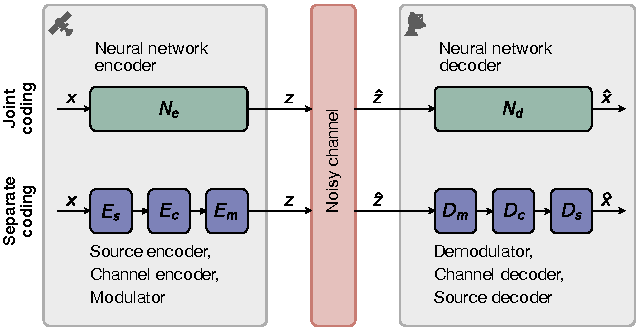
\includegraphics[width=\linewidth]{figures/coding-decoding}

  \caption{Overview of our communication architecture and comparison with traditional separate-encoder designs.}
  \label{fig:overview}
\end{figure}

To introduce our protocol's main components, we first explain the basic \ac{jscc} communication architecture and contrast it to the traditional case that uses separate encoders and decoders.
\Cref{fig:overview} shows an overview of the architecture in contrast to traditional approaches.
With separate coding (shown in the bottom half), the sensor data $x \in \mathbb{R}^n$ is first encoded using a source encoder, such as \jpegtwok.
Afterwards, a channel encoder (e.g., \ac{ldpc}) adds redundancy to the compressed signal in order to protect it against packet loss due to interference.
The modulator component then translates the channel encoder's output to physical layer samples $z \in \mathbb{C}^k$, which can be transmitted over a noisy channel.
The ground station receives the distorted signal $\hat{z}$ and uses corresponding components in inverse order to decode an approximation of $x$.
The demodulator $D_m$ translates the samples back to bits, which serve as input to the channel decoder $D_c$.
The channel decoder reconstructs the compressed image data, correcting transmission errors as far as possible.
The source decoder $D_s$ finally approximately reconstructs the original optical sensor data as $\hat{x}$.

In our \ac{jscc} approach (upper half of \Cref{fig:overview}), in contrast, parts of a single neuronal network are used as encoder $N_e$ and decoder $N_d$ by the satellite and ground station, respectively.
These components jointly perform the source coding, channel coding, modulation, and their corresponding inverse operations.

We use an encoder-decoder neuronal network architecture based on \cite{satjscc} to implement $N_e$ and $N_d$:
During training, the encoder ($N_e$) and decoder ($N_d$) parts of the network are linked together using a realistic channel model for noisy satellite links.
To better reflect realistic channel conditions, we replace the \ac{awgn} channel used in \cite{satjscc} with a more realistic channel model for \ac{leo} satellites.
The encoder-decoder model is then trained using an image dataset derived from the body of \sentinelii mission data.
The images within the dataset are used as model input and the reconstructed image's quality is used as reward metric.
Normally, a separate model would need to be trained for each characteristic set of channel conditions \cite{satjscc}.
In order to use a single network for a wide array of channel conditions, we augment the model with so-called attention modules \cite{wireless-attention-modules} as part of both the encoder and decoder during training.
These essentially allow to parameterize the network during later operation to cater to changing channel conditions.
The trained network is then separated into the encoder component $N_e$, which is used by the satellite and the decoder component $N_d$, which is used by the ground station.

\subsection{Encoder-decoder architecture with attention modules}

\begin{figure}
  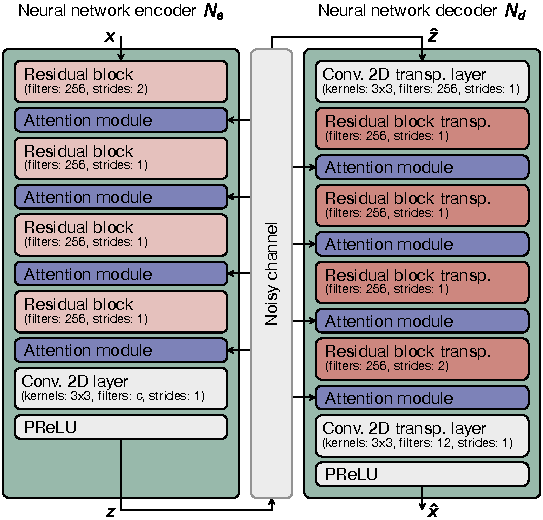
\includegraphics[width=\linewidth]{figures/network-architecture}

  \caption{Network architecture overview.}
  \label{fig:architecture-overview}
\end{figure}

The encoder-decoder network architecture is shown in \Cref{fig:architecture-overview}.
As basis, we use the network structure proposed in \cite{satjscc}, which adapts ResNet \cite{resnet} to the \ac{jscc} use case.
To make the architecture more flexible, we add attention modules, as well as a more realistic channel model.
The block on the left serves as neural network encoder, jointly performing source coding, channel coding, and modulation.
Compression is achieved by translating the input $x \in \mathbb{R}^n$ to channel symbols $z \in \mathbb{C}^k$, where $k < n$.
By adjusting $k$, the system's compression ratio $k/n$ can be defined.

\begin{figure*}
  \begin{subfigure}{.3\linewidth}
    \centering
    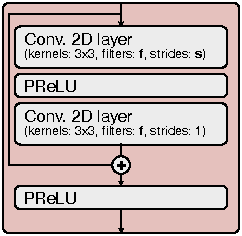
\includegraphics[height=10em]{figures/residual-block}
    \caption{Residual block $(f, s)$}
    \label{fig:residual}
  \end{subfigure}
  \hfill
  \begin{subfigure}{.3\linewidth}
    \centering
    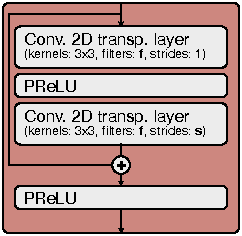
\includegraphics[height=10em]{figures/residual-block-transpose}
    \caption{Residual block transpose $(f, s)$}
    \label{fig:residual-transpose}
  \end{subfigure}
  \hfill
  \begin{subfigure}{.3\linewidth}
    \centering
    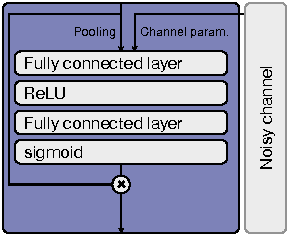
\includegraphics[height=10em]{figures/attention-module}
    \caption{Attention module}
    \label{fig:attention}
  \end{subfigure}

  \caption{Specific block architectures used within the encoder-decoder network.}
  \label{fig:blocks}
\end{figure*}

For the encoder, we use four residual blocks with 256 filters and a kernel size of $3 \times 3$.
The structure of the residual blocks is shown in \Cref{fig:residual}.
Each residual block is followed by an attention module as proposed in \cite{wireless-attention-modules}.
\Cref{fig:attention} shows the structure of the attention modules.
These modules allow to alter the feature weights of their preceding residual blocks in order to accommodate different channel conditions.
To do so, a number of channel parameters are added as additional input to the attention modules.
Based on these parameters, a number of scaling parameters are learned that either increase or decrease the connection strength to the next module, depending on the specific channel condition.
The attention modules operate in three steps.
First, global average pooling is applied to the previous residual block's output, which serves to make available global context information.
The pooled output is then concatenated with variables representing channel parameters.
Second, a simple neural network structure -- two fully connected layers plus \ac{relu} and sigmoid as activation functions -- is used to predict the proper scaling factors based on the channel condition parameters.
Finally, the previous residual layer's output is multiplied with the predicted scaling factors to implement the attention-based scaling.

As last layer of the encoder component, we use a convolutional layer that contains $c$ filters.
The value for $c$ is chosen based on the desired compression ratio $k/n$.
Finally, \ac{prelu} is used as activation function.
The result is a vector $\tilde{z}$ comprising $k$ complex numbers, which represent the channel symbols.

To learn and predict the actual channel conditions, the middle component of the encoder-decoder architecture ia a non-trainable channel layer, which models a realistic representation of the channel conditions in satellite communication.
For the channel, we assume a log-normal distribution with mean $\alpha$ and standard deviation $\psi$, a Rayleigh-distributed multi-path component \MP, and a signal-to-noise parameter \SNR.
We present the channel model in more detail in \Cref{sub:channel_model}.

The block on the right serves as neural network decoder, which translates the -- potentially corrupted channel symbols $\hat{z}$ back to an approximation $\hat{x}$ of the original data.
The decoder follows the same architecture design as the encoder: a convolutional transpose layer is followed by four residual transpose blocks plus corresponding attention modules,  another convolutional transpose layer, and a \ac{prelu} activation function.

As reward function during model training and to evaluate the quality of the reconstructed image signal, we use the \ac{psnr} metric:
%
\begin{equation}
  \mathrm{PSNR} = 10 \log_{10}\frac{\mathrm{MAX}^2}{\mathrm{MSE}},
\end{equation}
%
where $\mathrm{MAX}$ is the maximum possible pixel value.
The \ac{psnr} captures to what extent original signal value is affected by distorting noise as a fraction between the maximum signal and noise.


\subsection{Channel model for \ac{leo} satellites}
\label{sub:channel_model}

We compute the channel output symbols $\hat{z}$ as follows:
\begin{equation}
  \hat{z} = zh + n,
\end{equation}
where $h$ denotes channel gain and $n$ Gaussian noise.
Next, we explain how $h$ and $n$ are calculated.

To account for specific satellite channel conditions, we compute $h$ using Fontan's statistical channel~\cite{} model. 
Since the satellite channel characteristics heavily depend on shadowing conditions, in general, 
they cannot be accurately modeled using a single distribution.
Typically, multiple states describing different degrees of scheduling are introduced 
and the overall pdf is given as a sum of of the individual state pdfs multiplied by the probabilities of being in a given state.
For example, assuming a two-state model with \ac{los} and shadow conditions: 
\begin{equation}
f_{\mathrm{overall}}(r) = p_{\mathrm{los}}f_{\mathrm{los}}(r) + p_{\mathrm{shadow}}f_{\mathrm{shadow}}(r)
\end{equation}

Furthermore, to add more details, e.g. state duration, Markov chain models can be introduced.
Then, the propagation channel at a given time is described by the state probability matrix, which contains the of being in a particular state
and the state transition probability matrix, which contains the probability of changing from state $i$ to state $j$.

The Fontan's channel model is a three-state Markov chain model containing the following states:
\begin{itemize}
  \item \ac{los} (no shadowing)
  \item shadow (moderate shadowing conditions)
  \item deep shadow (heavy shadowing conditions)
\end{itemize}

In each state, the channel is modeled using Loo distribution~\cite{}. 
The overall received signal is described as a sum of the log-normally distributed direct component and Rayleigh distributed multipath component with parameters $\alpha$, $\psi$ and \MP.
The log-normal distribution is characterized by mean $\alpha$ and standard deviation $\psi$ and Rayleigh distribution by its average power \MP.
Different values for $\alpha$, $\psi$ and \MP are chosen depending on the state and elevation angle.
The \ac{pdf} is as follows:
\begin{equation}
  \begin{aligned}
  p(r) &= \frac{r}{b_0\sqrt{2\pi d_0}} \\[1ex]
  &\hphantom{=} \cdot \int_{0}^{\infty}\frac{1}{z} \exp\left[-\frac{(\ln z - \mu)^2}{2d_0} - \frac{r^2 + z^2}{2b_0}\right] \\[1ex]
  &\hphantom{=\int_{0}^{\infty}} \cdot I_0\Big(\frac{rz}{b_0}\Big)\ dz
  \end{aligned}
\end{equation}

whereby there the following dependencies exist between $mu$, $d_0$ and $b_0$ and $\alpha$, $\psi$ and \MP:
\begin{align}
\alpha &= 20\log_{10}(e^\mu) \\
  \psi &= 20\log_{10}(e^{\sqrt{d_0}}) \\
   \MP &= 10\log_{10}(2b_0)
\end{align}

Next, we consider the Gaussian noise $n$. We follow the approach presented in~\cite{LCN23}. 
We first compute the typical \ac{snr} values. 
To this end, we determine the distance $d$ between the satellite and the ground station based on the current elevation angle $\epsilon_0$ and Earth radius $R_E = 6378\,\textrm{km}$ as described in \cite{}:
%
\begin{equation}
  d = R_E\Biggl(\sqrt{\Bigl(\frac{h + R_E}{R_E}\Bigr)^2 - \cos^{2}\epsilon_{0}} - \sin\epsilon_{0}\Biggr),
\end{equation}
%

Next, we compute thermal noise $N$ as follows:
%
\begin{equation}
  N=k \cdot T \cdot B,
\end{equation}
%
where $B$ and $T$ denote the bandwidth and noise temperature respectively and $k = 1.380649 \cdot 10^{-23}$ is the Boltzmann's constant.
We compute the noise temperature as the sum of the antenna temperature $T_a = 290 K$ and the receiver noise temperature $T_e$, which is determined as:
%
\begin{equation}
  T_e = T_0 \big(F_{\mathrm{sys}} - 1 \big),
\end{equation}
%
$T_0 = 290$\,K is the reference temperature and $F_{\textrm{sys}} = 2$\,dB denotes the receiver's noise figure.

Next, we compute the path loss $L$ using the Friis formula \cite{} and determine the SNR depending on $L$ and $N$ as follows:
%
\begin{equation}
  \mathrm{SNR} = P_t + G_t + G_r - L - N,
\end{equation}
%
where $P_t$, $G_t$ and $G_r$ are input parameters denoting the transmitted power, the transmitter and the receiver gains respectively. 
The computed $\mathrm{SNR}$ value is then used to compute the noise power $\sigma^2$:
%
\begin{equation}
  \sigma^2 = \frac{P_{\mathrm{sig}}}{2 \cdot 10^{\frac{\mathrm{SNR}}{10}}}
\end{equation}
%
where $P_{\mathrm{sig}}$ is the normalized signal power.
Finally, we compute the noise vector $n$ as follows:
%
\begin{equation}
  n = \sigma \times \bigl[\mathcal{N}(0,1) + j * \mathcal{N}(0,1) \bigr] 
\end{equation}
%

%TODO:
% - z ersetzen weil doppelt
% - r, b0, d0, z erklären
% - Formel für h

\section{Evaluation}
\label{sec:evaluation}

\begin{table}
  \caption{Channel Parameters}
  \label{tab:channel_parameters}

  \centering
	\begin{tabular}{ll}
		\toprule
    Parameter & Value \\
    \midrule
		Orbit height & 150\,km \\
		Carrier frequency & 2150\,MHz \\
    Transmitted power & 1\,W \\
    Satellite antenna gain & 6\,dBi \\
    Ground station antenna gain & 35\,dBi \\
		Receive channel bandwidth & 750\,kHz \\
		Noise figure & 2\,dB \\
		\bottomrule
	\end{tabular}
\end{table}

%%% FROM LAST YEAR %%%

In this section, we evaluate the \ac{jscc-sat} approach by comparing it to \jpegtwok, 
which is commonly used for compression of satellite images~\cite{sentinel-2-user-handbook}.
We use the BigEarth dataset~\cite{sumbul2019bigearthnet,Sumbul2021}, which is a collection of 590,326 multi-spectral images acquired by \sentinelii, as explained in \Cref{sub:eo}.
More specifically, we use a subset of all images contained in the dataset, which cover the area of Serbia in the summer months.
We remove cloudy images from the dataset with the help of a script provided by the BigEarthNet authors, following common evaluation practices.
In total, 14,439 multi-spectral images remain in the filtered dataset.
Each multi-spectral image is represented by 12 individual files, where each file encodes one of the bands using the lossless \ac{tiff} format.
The dataset was then further divided into training, validation, and test sets.
Since the individual bands in the dataset have different resolutions (see \Cref{tab:sentinel_bands}), we used cubic interpolation to resize all image files to the same size.
The dataset contains 12 bands. \sentinelii's band 10 contains information about clouds is not included in the dataset, since it is not useful for training.
Finally, the pixel values were normalized so that they are between 0 and 1.

To apply \ac{jscc-sat}, we implement the neural network architecture described in \Cref{sec:jscc} using Keras\footnote{Website: https://keras.io/} and Tensorfow.\footnote{Website: https://www.tensorflow.org/}
The batch size was set to 32, and the learning rate was set to $10^{-3}$ and adjusted to $10^{-4}$ after 500 epochs.
We used Adam as optimizer, which is a form of stochastic gradient descent.
A separate neural network was trained till convergence for each SNR value.

We further computed the \ac{snr} values using the formulas described in \Cref{sub:link_budget} and the parameters from \Cref{tab:channel_parameters}.
As main varying factor, we consider the satellites elevation angle relative to the ground station to cover a wide range of possible transmission environments.
\Cref{fig:snr_elevation} shows the \acp{snr} depending on the elevation angle.
A separate neural network is trained for each \ac{snr} value.

We consider two simulation scenarios:
%
\begin{enumerate}
  \item We compare \ac{jscc-sat} against \jpegtwok with maximum rate for source compression, that is, assuming guaranteed reliable transmission according to Shannon's separation theorem, to obtain an upper bound for the performance of \jpegtwok.
  \item We compare \ac{jscc-sat} against \jpegtwok with additional channel coding using \ac{ldpc} for a more realistic upper bound.
\end{enumerate}

For both scenarios, we compare the achieved image quality measured using \ac{psnr} values for various realistic \ac{snr} values.
The higher the \ac{psnr} values of the reconstructed images, the better the image quality.

%%% END FROM LAST YEAR %%%


In this section, we evaluate \ours and compare the results against multiple neural networks trained individually for each parameter set.
We evaluate using statistical data from \cite{channel_values}. 
They provide values for $\alpha$, $\psi$ and \MP for five different environments (open, suburban, intermediate tree-shadow, heavy tree-shadow, urban).
The measurements were conducted for 40, 60, 70, and 80 elevation angles.
Three states describing different shadowing conditions are introduced: line-of-sight (LOS), intermediate shadow, and deep shadow.
First, we evaluate how JSCC without AF performs on the data to identify how various parameter combinations influence the results.
We consider different environments, states, compression ratios and elevation angles. 
Then we compare the performance of \ours against JSCC.
Finally, we compare \ours against JSCC in the case of state mismatch, i.e. when the actual channel state differs from what we expected.

\begin{figure*}[t!]
  \begin{subfigure}{.32\linewidth}
  \centering
  \begin{tikzpicture}
    \begin{axis}[
        width=\linewidth,
        height=.65\linewidth,
        xlabel = {Compression ratio},
        ylabel = {PSNR},
        ymin = 50,
        ymax = 70,
        ylabel near ticks,
        xtick = data,
        x tick label style={
            rotate=45,
            /pgf/number format/fixed,
            /pgf/number format/precision=2,
        },
        x label style={below=0},
        ]

        \addplot[mark=triangle*,plt1] 
        plot 
        table[x expr=\thisrowno{0}, y expr=\thisrowno{1}, col sep=space] {plots/no_AF_40_open_los_los};

        \addplot[mark=triangle*,plt2] 
        plot 
        table[x expr=\thisrowno{0}, y expr=\thisrowno{1}, col sep=space] {plots/no_AF_40_suburban_los_los};

        \addplot[mark=triangle*,plt3] 
        plot 
        table[x expr=\thisrowno{0}, y expr=\thisrowno{1}, col sep=space] {plots/no_AF_40_intermediate_tree_shadow_los_los};
        
%         \addplot[tol4!60, thick] 
%         plot 
%         table[x expr=\thisrowno{0}, y expr=\thisrowno{1}, col sep=space] {../results/no_AF_40_heavy_tree_shadow_shadow_shadow};
        
        \addplot[mark=triangle*,plt5] 
        plot 
        table[x expr=\thisrowno{0}, y expr=\thisrowno{1}, col sep=space] {plots/no_AF_40_urban_los_los};


%         \legend{
%             open,
%             suburban, 
%             intermediate tree shadow,
% %             heavy tree shadow,
%             urban
%             }


    \end{axis}
\end{tikzpicture}

  \caption{LOS}
\end{subfigure}
\hfill
\begin{subfigure}{.32\linewidth}
  \centering
  \begin{tikzpicture}
    \begin{axis}[
        width=\linewidth,
        height=.7\linewidth,
        xlabel = {Compression ratio},
        ylabel = {PSNR},
        ymin = 50.0,
        ymax = 70,
        ylabel near ticks,
        xtick = data,
        x tick label style={
            rotate=45,
            /pgf/number format/fixed,
            /pgf/number format/precision=2,
        },
        x label style={below=1em},
        legend cell align={left},
        legend columns=5,
		legend style={/tikz/every even column/.append style={column sep=1em}},
        legend to name={legendenv},
        ]

        \addplot[mark=triangle*,plt1] 
        plot 
        table[x expr=\thisrowno{0}, y expr=\thisrowno{1}, col sep=space] {plots/no_AF_40_open_shadow_shadow};

        \addplot[mark=triangle*,plt2] 
        plot 
        table[x expr=\thisrowno{0}, y expr=\thisrowno{1}, col sep=space] {plots/no_AF_40_suburban_shadow_shadow};

        \addplot[mark=triangle*,plt3] 
        plot 
        table[x expr=\thisrowno{0}, y expr=\thisrowno{1}, col sep=space] {plots/no_AF_40_intermediate_tree_shadow_deep_shadow_deep_shadow};
        
        \addplot[mark=triangle*,plt4] 
        plot 
        table[x expr=\thisrowno{0}, y expr=\thisrowno{1}, col sep=space] {plots/no_AF_40_heavy_tree_shadow_shadow_shadow};
        
        \addplot[mark=triangle*,plt5] 
        plot 
        table[x expr=\thisrowno{0}, y expr=\thisrowno{1}, col sep=space] {plots/no_AF_40_urban_shadow_shadow};


        \legend{
            open,
            suburban, 
            intermediate tree shadow,
            heavy tree shadow,
            urban
            }


    \end{axis}
\end{tikzpicture}

  \caption{Shadow}
\end{subfigure}
\hfill
\begin{subfigure}{.32\linewidth}
  \centering
  \begin{tikzpicture}
    \begin{axis}[
        width=\linewidth,
        height=.65\linewidth,
        xlabel = {Compression ratio},
        ylabel = {PSNR},
        ymin = 50,
        ymax = 70,
        ylabel near ticks,
        xtick = data,
        x tick label style={
            rotate=45,
            /pgf/number format/fixed,
            /pgf/number format/precision=2,
        },
        x label style={below=0},
        ]

        \addplot[mark=triangle*,plt1] 
        plot 
        table[x expr=\thisrowno{0}, y expr=\thisrowno{1}, col sep=space] {plots/no_AF_40_open_deep_shadow_deep_shadow};

        \addplot[mark=triangle*,plt2] 
        plot 
        table[x expr=\thisrowno{0}, y expr=\thisrowno{1}, col sep=space] {plots/no_AF_40_suburban_deep_shadow_deep_shadow};

        \addplot[mark=triangle*,plt3] 
        plot 
        table[x expr=\thisrowno{0}, y expr=\thisrowno{1}, col sep=space] {plots/no_AF_40_intermediate_tree_shadow_deep_shadow_deep_shadow};
        
        \addplot[mark=triangle*,plt4] 
        plot 
        table[x expr=\thisrowno{0}, y expr=\thisrowno{1}, col sep=space] {plots/no_AF_40_heavy_tree_shadow_deep_shadow_deep_shadow};
        
        \addplot[mark=triangle*,plt5] 
        plot 
        table[x expr=\thisrowno{0}, y expr=\thisrowno{1}, col sep=space] {plots/no_AF_40_urban_deep_shadow_deep_shadow};


        % \legend{
        %     open,
        %     suburban, 
        %     intermediate tree shadow,
        %     heavy tree shadow,
        %     urban
        %     }


    \end{axis}
\end{tikzpicture}

  \caption{Deep shadow}
\end{subfigure}

\vspace{1em}
\centering
\ref{legendenv}

\caption{No AF, different environments, 40 elevation angle}
\label{fig:different_scenes_40}
\end{figure*}

The results for 40 elevation angle are presented in \Cref{fig:different_scenes_40}. 
The x-axis shows different compression rates and y-axis the achieved PSNR values.
It can be seen that the results strongly depend on the environment.
As expected, the best PSNR values are achieved by open and the worse for much more challenging environments such as urban or intermediate tree-shadow.
It also can be seen that the results significantly depend on shadowing conditions. 
While for deep shadow the performance varies considerably between different environments, 
the differences become less pronounced as shadowing conditions improve.



\begin{figure*}[t!]
  \begin{subfigure}{.32\linewidth}
  \centering
  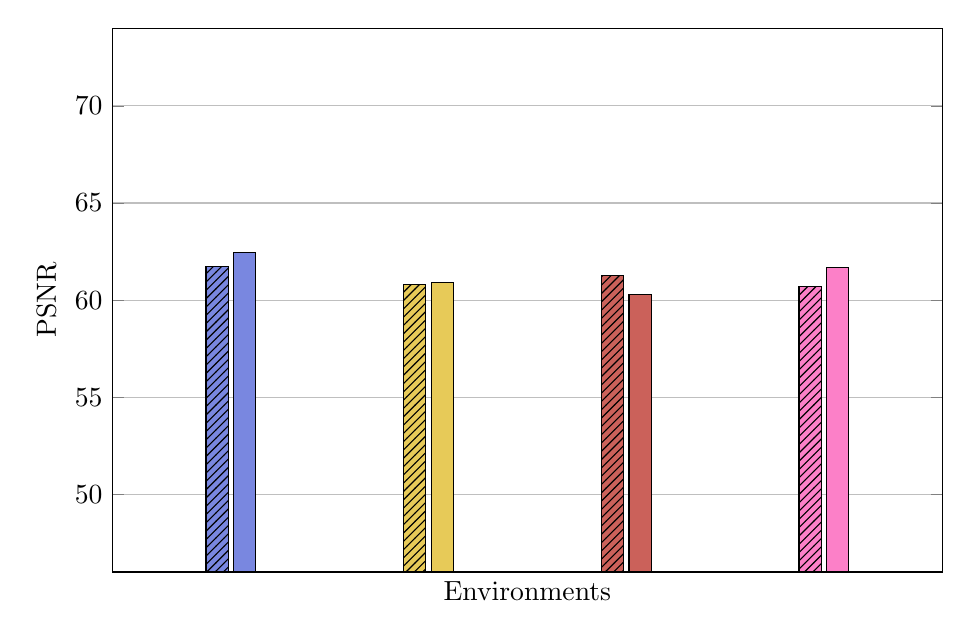
\begin{tikzpicture}
    \begin{axis}[
      ybar,
      width=\linewidth,
      height=.7\linewidth,
      ylabel near ticks,
      xlabel near ticks,
      xmajorticks=false,
      every axis plot/.append style={
                bar width=8pt,
                bar shift=0pt,
                fill
              },
      ymajorgrids=true,
      ylabel={PSNR},
      ymin=50,
      ymax=70,
      enlargelimits=.2,
      xlabel={Environments},
      symbolic x coords ={%
          open,
          suburban,
          intermediate tree-shadow,
          urban,
      },
      legend cell align={left},
      legend style={column sep=5pt},
      legend to name={legendangles},
      legend columns=2,
      xticklabel=\empty,
      ]
      
      \legend{
        40,
        80
      }

      \addplot[
        bar shift=-5pt,fill=white,postaction={
        pattern=north east lines, pattern color=black
    }] coordinates { (open, 0) };
      \addplot[bar shift=5pt,fill=white] coordinates { (open, 0) };

      \addplot[
        bar shift=-5pt,fill=plt1!70,postaction={
        pattern=north east lines, pattern color=black
    }] coordinates { (open, 61.73067188214748) };
      \addplot[bar shift=5pt,fill=plt1!70] coordinates { (open, 62.46548778477633) };
      

      \addplot[
      bar shift=-5pt,fill=plt2!70,postaction={
        pattern=north east lines, pattern color=black
    }] coordinates { (suburban, 60.805258435946925) };
      \addplot[bar shift=5pt,fill=plt2!70] coordinates { (suburban, 60.92828818309016) };
      
      \addplot[
        bar shift=-5pt,fill=plt3!70,postaction={
        pattern=north east lines, pattern color=black
    }] coordinates { (intermediate tree-shadow, 61.2610153054711) };
      \addplot[bar shift=5pt,fill=plt3!70] coordinates { (intermediate tree-shadow, 60.29798046606024) };
      
      \addplot[
        bar shift=-5pt,fill=plt5!70,postaction={
        pattern=north east lines, pattern color=black
    }] coordinates { (urban, 60.67812370860495) };
      \addplot[bar shift=5pt,fill=plt5!70] coordinates { (urban, 61.670784487418885) };
      
    \end{axis} 
  \end{tikzpicture}
  \caption{LOS, comp 0.04}
\end{subfigure}
\hfill
\begin{subfigure}{.32\linewidth}
  \centering
  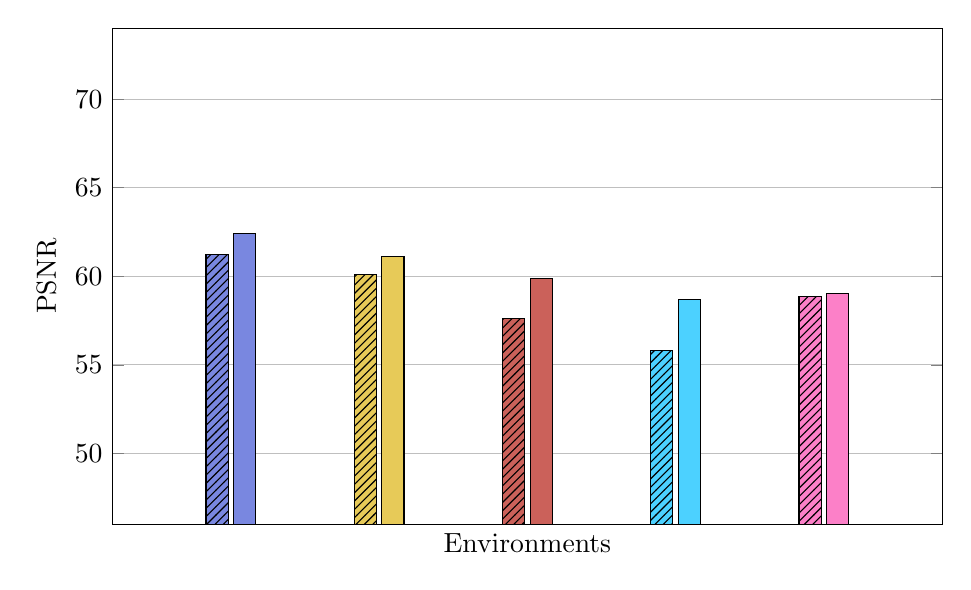
\begin{tikzpicture}
    \begin{axis}[
      ybar,
      width=\linewidth,
      height=.65\linewidth,
      ylabel near ticks,
      xlabel near ticks,
      xmajorticks=false,
      every axis plot/.append style={
                bar width=8pt,
                bar shift=0pt,
                fill
              },
      ymajorgrids=true,
      ylabel={PSNR},
      ymin=50,
      ymax=70,
      enlargelimits=.2,
      xlabel={Environments},
      symbolic x coords ={%
          open,
          suburban,
          intermediate tree-shadow,
          heavy tree-shadow,
          urban,
      },
      xticklabel=\empty,
      ]
  
      \addplot[
        bar shift=-5pt,fill=white,postaction={
        pattern=north east lines, pattern color=black
    }] coordinates { (open, 0) };
      \addplot[bar shift=5pt,fill=white] coordinates { (open, 0) };

      \addplot[
        bar shift=-5pt,fill=plt1!70,postaction={
        pattern=north east lines, pattern color=black
    }] coordinates { (open, 61.242307462063216) };
      \addplot[bar shift=5pt,fill=plt1!70] coordinates { (open, 62.43216132742652) };
      

      \addplot[
      bar shift=-5pt,fill=plt2!70,postaction={
        pattern=north east lines, pattern color=black
    }] coordinates { (suburban, 60.0867862998761) };
      \addplot[bar shift=5pt,fill=plt2!70] coordinates { (suburban, 61.12110295624692) };
      
      \addplot[
        bar shift=-5pt,fill=plt3!70,postaction={
        pattern=north east lines, pattern color=black
    }] coordinates { (intermediate tree-shadow, 57.62850182792831) };
      \addplot[bar shift=5pt,fill=plt3!70] coordinates { (intermediate tree-shadow, 59.88167207543309) };
      
      \addplot[
        bar shift=-5pt,fill=plt4!70,postaction={
        pattern=north east lines, pattern color=black
    }] coordinates { (heavy tree-shadow, 55.79653619027105) };
      \addplot[bar shift=5pt,fill=plt4!70] coordinates { (heavy tree-shadow, 58.7045005554619) };
      
      \addplot[
        bar shift=-5pt,fill=plt5!70,postaction={
        pattern=north east lines, pattern color=black
    }] coordinates { (urban, 58.862160183144205) };
      \addplot[bar shift=5pt,fill=plt5!70] coordinates { (urban, 59.03699565522086) };
      
    \end{axis} 
  \end{tikzpicture}
  \caption{Shadow, comp 0.04}
\end{subfigure}
\hfill
\begin{subfigure}{.32\linewidth}
  \centering
  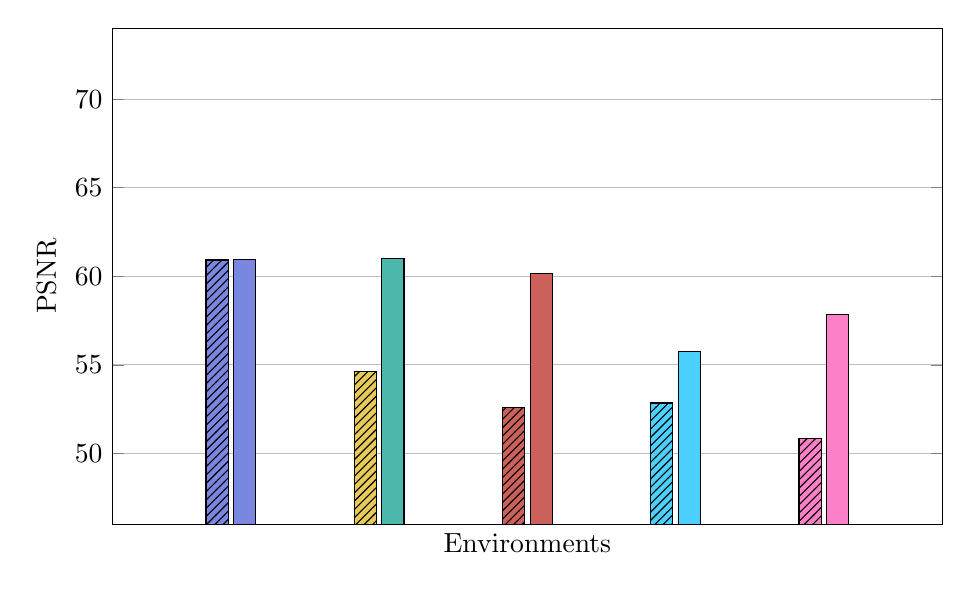
\begin{tikzpicture}
    \begin{axis}[
      ybar,
      width=\linewidth,
      height=.65\linewidth,
      ylabel near ticks,
      xlabel near ticks,
      xmajorticks=false,
      every axis plot/.append style={
                bar width=8pt,
                bar shift=0pt,
                fill
              },
      ymajorgrids=true,
      ylabel={PSNR},
      ymin = 50,
        ymax = 70,
      enlargelimits=.2,
      xlabel={Environments},
      symbolic x coords ={%
          open,
          suburban,
          intermediate tree-shadow,
          heavy tree-shadow,
          urban,
      },
      xticklabel=\empty,
      ]
  
      \addplot[
        bar shift=-5pt,fill=white,postaction={
        pattern=north east lines, pattern color=black
    }] coordinates { (open, 0) };
      \addplot[bar shift=5pt,fill=white] coordinates { (open, 0) };

      \addplot[
        bar shift=-5pt,fill=plt1!70,postaction={
        pattern=north east lines, pattern color=black
    }] coordinates { (open, 60.915204772562106) };
      \addplot[bar shift=5pt,fill=plt1!70] coordinates { (open, 60.941951355437276) };
      

      \addplot[
      bar shift=-5pt,fill=plt2!70,postaction={
        pattern=north east lines, pattern color=black
    }] coordinates { (suburban, 54.626502435886835) };
      \addplot[bar shift=5pt,fill=tol2!70] coordinates { (suburban, 61.017142451016966) };
      
      \addplot[
        bar shift=-5pt,fill=plt3!70,postaction={
        pattern=north east lines, pattern color=black
    }] coordinates { (intermediate tree-shadow, 52.57299641191118) };
      \addplot[bar shift=5pt,fill=plt3!70] coordinates { (intermediate tree-shadow, 60.14165345147827) };
      
      \addplot[
        bar shift=-5pt,fill=plt4!70,postaction={
        pattern=north east lines, pattern color=black
    }] coordinates { (heavy tree-shadow, 52.84660367941581) };
      \addplot[bar shift=5pt,fill=plt4!70] coordinates { (heavy tree-shadow, 55.73117874454389) };
      
      \addplot[
        bar shift=-5pt,fill=plt5!70,postaction={
        pattern=north east lines, pattern color=black
    }] coordinates { (urban, 50.84575762551614) };
      \addplot[bar shift=5pt,fill=plt5!70] coordinates { (urban, 57.86157808541486) };
      
    \end{axis} 
  \end{tikzpicture}
  \caption{Deep shadow, comp 0.04}
\end{subfigure}

\vspace{1em}

\begin{subfigure}{.32\linewidth}
  \centering
  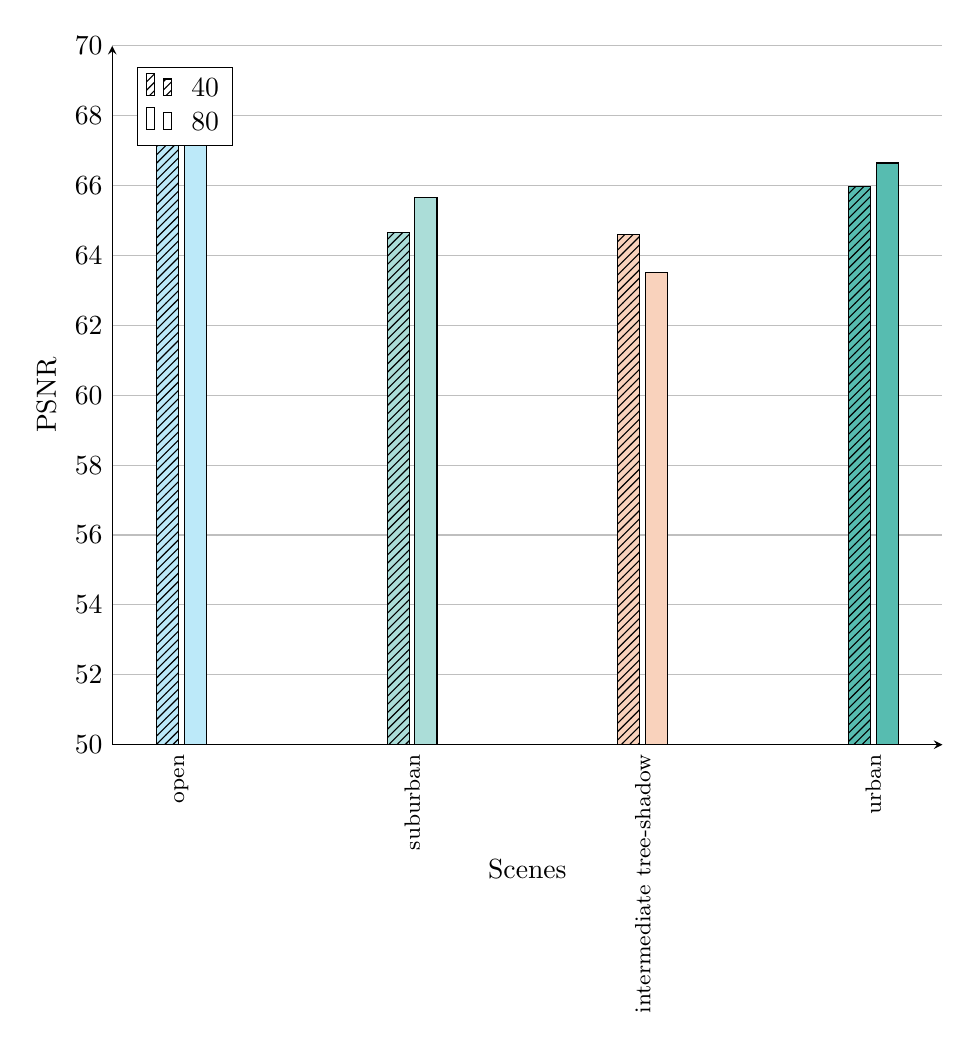
\begin{tikzpicture}
    \edef\mylst{"An arbitrary string","String","Custom label","Not this data"}
    \begin{axis}[
      ybar,
      %log ticks with fixed point,
      width=\linewidth,
      %height=.5\linewidth,
      every axis plot/.append style={
                %ybar,
                bar width=8pt,
                bar shift=0pt,
                fill
              },
      %
      % nodes near coords,
      % nodes near coords align=above,
      % nodes near coords align={vertical},
      xtick={%
          \null,
          open,  suburban,  intermediate tree-shadow,
          urban,
      },
      %
      axis x line=bottom,
      axis y line=left,
      ymajorgrids=true,
      %
      ylabel={PSNR},
      %y label style={at={(axis description cs:0.1,.3)},anchor=south},
      ymin=50,
      ymax=70,
      enlargelimits=auto,
      %
      xlabel={Scenes},
      %
      nodes near coords align=above,
        every node near coord/.append style={xshift=5pt},
      %
      symbolic x coords ={%
          \null,
          open,  suburban,  intermediate tree-shadow,
          urban,
          % \null
      },
      legend cell align={left},
      legend style={column sep=5pt},
      legend pos=north west,
      %y coord trafo/.code={\pgfmathparse{#1 * 0.000001}},
      x tick label style={font=\footnotesize,rotate=90,anchor=east,major tick length=0pt},
        x label style={at={(axis description cs:0.5,-0.15)},anchor=north},
      ]
  
      %\addplot[fill=tol1!33] coordinates { (4/64, 2758668.0) (8/64, 1379334.0) (16/64, 689667.0) (4/128, 3218446.0) (8/128, 1609223.0) (16/128, 804611.5) (4/256, 3678224.0) (8/256, 1839112.0) (16/256, 919556.0) (4/512, 4138002.0) (8/512, 2069001.0) (16/512, 1034500.5)};
      %\addplot[fill=tol2!33] coordinates { (4/64, 2067667.375)  (8/64, 1188627.125) (16/64, 590885.25) (4/128, 2596351.875) (8/128, 1396883.625) (16/128, 710855.0) (4/256, 3006822.875) (8/256, 1475599.875) (16/256, 820431.75) (4/512, 3445006.625) (8/512, 1681019.375) (16/512, 908686.125)};
      
      \legend{
        40,
        80
      }

      \addplot[
        bar shift=-5pt,fill=white,postaction={
        pattern=north east lines, pattern color=black
    }] coordinates { (open, 0) };
      \addplot[bar shift=5pt,fill=white] coordinates { (open, 0) };

      \addplot[%nodes near coords=$1.36$,
        bar shift=-5pt,fill=tol1!33,postaction={
        pattern=north east lines, pattern color=black
    }] coordinates { (open, 67.22762412790338) };
      \addplot[bar shift=5pt,fill=tol1!33] coordinates { (open, 67.94286665070874) };
      

      \addplot[%nodes near coords=$1.18$,
      bar shift=-5pt,fill=tol2!33,postaction={
        pattern=north east lines, pattern color=black
    }] coordinates { (suburban, 64.65365825355423) };
      \addplot[bar shift=5pt,fill=tol2!33] coordinates { (suburban, 65.65526368893802) };
      
      \addplot[%nodes near coords=$1.19$,
        bar shift=-5pt,fill=tol3!33,postaction={
        pattern=north east lines, pattern color=black
    }] coordinates { (intermediate tree-shadow, 64.59177795781159) };
      \addplot[bar shift=5pt,fill=tol3!33] coordinates { (intermediate tree-shadow, 63.51533179513708) };
      
      \addplot[%nodes near coords=$1.17$,
        bar shift=-5pt,fill=tol2!66,postaction={
        pattern=north east lines, pattern color=black
    }] coordinates { (urban, 65.96625190247083) };
      \addplot[bar shift=5pt,fill=tol2!66] coordinates { (urban, 66.64719138769036) };
      
    \end{axis} 
  \end{tikzpicture}
  \caption{LOS, comp 0.33}
\end{subfigure}
\hfill
\begin{subfigure}{.32\linewidth}
  \centering
  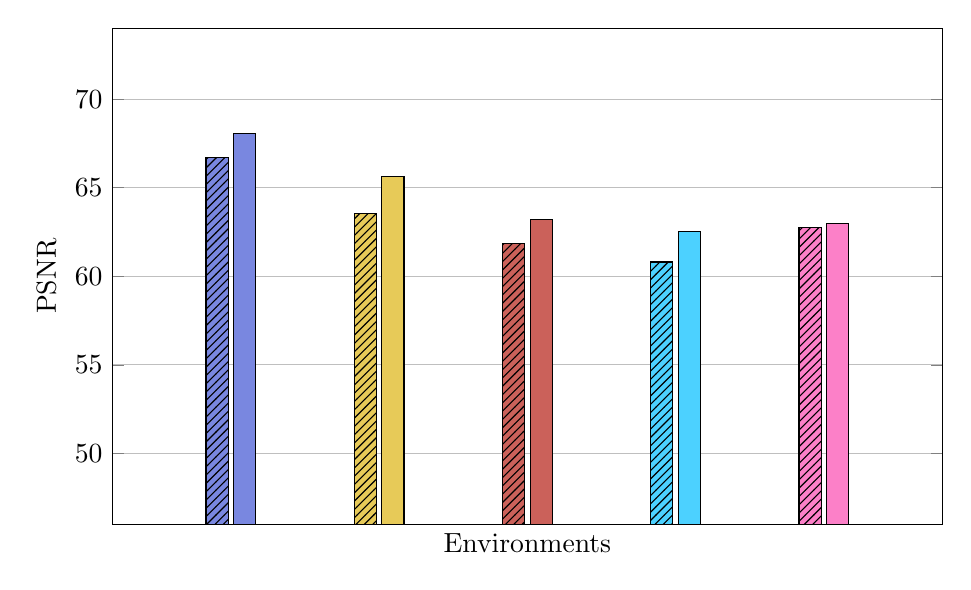
\begin{tikzpicture}
    \begin{axis}[
      ybar,
      width=\linewidth,
      height=.65\linewidth,
      ylabel near ticks,
      xlabel near ticks,
      xmajorticks=false,
      every axis plot/.append style={
                bar width=8pt,
                bar shift=0pt,
                fill
              },
      ymajorgrids=true,
      ylabel={PSNR},
      ymin=50,
      ymax=70,
      enlargelimits=.2,
      xlabel={Environments},
      symbolic x coords ={%
          open,
          suburban,
          intermediate tree-shadow,
          heavy tree-shadow,
          urban,
      },
      xticklabel=\empty,
      ]

      \addplot[
        bar shift=-5pt,fill=white,postaction={
        pattern=north east lines, pattern color=black
    }] coordinates { (open, 0) };
      \addplot[bar shift=5pt,fill=white] coordinates { (open, 0) };

      \addplot[%nodes near coords=$1.36$,
        bar shift=-5pt,fill=plt1!70,postaction={
        pattern=north east lines, pattern color=black
    }] coordinates { (open, 66.72378601897488) };
      \addplot[bar shift=5pt,fill=plt1!70] coordinates { (open, 68.05071847613172) };
      

      \addplot[%nodes near coords=$1.18$,
      bar shift=-5pt,fill=plt2!70,postaction={
        pattern=north east lines, pattern color=black
    }] coordinates { (suburban, 63.5362946198049) };
      \addplot[bar shift=5pt,fill=plt2!70] coordinates { (suburban, 65.61713528754578) };
      
      \addplot[%nodes near coords=$1.19$,
        bar shift=-5pt,fill=plt3!70,postaction={
        pattern=north east lines, pattern color=black
    }] coordinates { (intermediate tree-shadow, 61.85098102603866) };
      \addplot[bar shift=5pt,fill=plt3!70] coordinates { (intermediate tree-shadow, 63.182928753310684) };
      
      \addplot[%nodes near coords=$1.26$,
        bar shift=-5pt,fill=plt4!70,postaction={
        pattern=north east lines, pattern color=black
    }] coordinates { (heavy tree-shadow, 60.80235241808859) };
      \addplot[bar shift=5pt,fill=plt4!70] coordinates { (heavy tree-shadow, 62.51972868765633) };
      
      \addplot[%nodes near coords=$1.17$,
        bar shift=-5pt,fill=plt5!70,postaction={
        pattern=north east lines, pattern color=black
    }] coordinates { (urban, 62.73554608081638) };
      \addplot[bar shift=5pt,fill=plt5!70] coordinates { (urban, 62.9654737199328) };
      
    \end{axis} 
  \end{tikzpicture}
  \caption{Shadow, comp 0.33}
\end{subfigure}
\hfill
\begin{subfigure}{.32\linewidth}
  \centering
  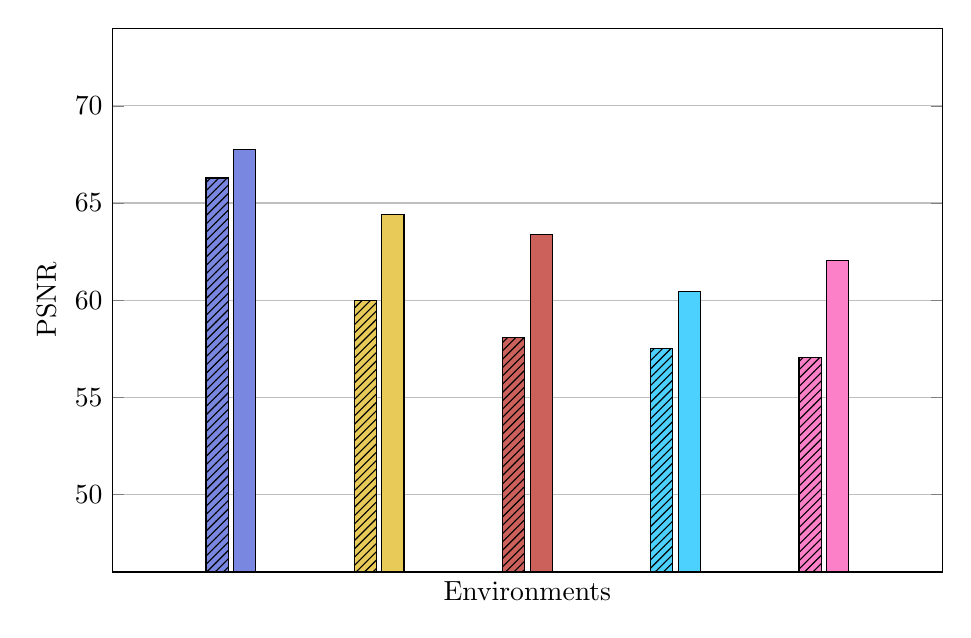
\begin{tikzpicture}
    \begin{axis}[
      ybar,
      width=\linewidth,
      height=.7\linewidth,
      ylabel near ticks,
      xlabel near ticks,
      xmajorticks=false,
      every axis plot/.append style={
                bar width=8pt,
                bar shift=0pt,
                fill
              },
      ymajorgrids=true,
      ylabel={PSNR},
      ymin=50,
      ymax=70,
      enlargelimits=.2,
      xlabel={Environments},
      symbolic x coords ={%
          open,
          suburban,
          intermediate tree-shadow,
          heavy tree-shadow,
          urban,
      },
      xticklabel=\empty,
      ]

      \addplot[
        bar shift=-5pt,fill=white,postaction={
        pattern=north east lines, pattern color=black
    }] coordinates { (open, 0) };
      \addplot[bar shift=5pt,fill=white] coordinates { (open, 0) };

      \addplot[%nodes near coords=$1.36$,
        bar shift=-5pt,fill=plt1!70,postaction={
        pattern=north east lines, pattern color=black
    }] coordinates { (open, 66.28719931983984) };
      \addplot[bar shift=5pt,fill=plt1!70] coordinates { (open, 67.76665563361574) };
      

      \addplot[%nodes near coords=$1.18$,
      bar shift=-5pt,fill=plt2!70,postaction={
        pattern=north east lines, pattern color=black
    }] coordinates { (suburban, 59.97375970276803) };
      \addplot[bar shift=5pt,fill=plt2!70] coordinates { (suburban, 64.41231830717751) };
      
      \addplot[%nodes near coords=$1.19$,
        bar shift=-5pt,fill=plt3!70,postaction={
        pattern=north east lines, pattern color=black
    }] coordinates { (intermediate tree-shadow, 58.080011031063236) };
      \addplot[bar shift=5pt,fill=plt3!70] coordinates { (intermediate tree-shadow, 63.39092156973394) };
      
      \addplot[%nodes near coords=$1.26$,
        bar shift=-5pt,fill=plt4!70,postaction={
        pattern=north east lines, pattern color=black
    }] coordinates { (heavy tree-shadow, 57.512479690636944) };
      \addplot[bar shift=5pt,fill=plt4!70] coordinates { (heavy tree-shadow, 60.45771389019385) };
      
      \addplot[%nodes near coords=$1.17$,
        bar shift=-5pt,fill=plt5!70,postaction={
        pattern=north east lines, pattern color=black
    }] coordinates { (urban, 57.03474187203291) };
      \addplot[bar shift=5pt,fill=plt5!70] coordinates { (urban, 62.0518730036318) };
      
    \end{axis} 
  \end{tikzpicture}
  \caption{Deep shadow, comp 0.33}
\end{subfigure}

\vspace{1em}
\centering
\ref{legendangles}
\tikz{%
  \node[draw=black, inner sep=3.55pt] {
    \tikz{\node[fill=plt1] {};} open \hspace{1em}
    \tikz{\node[fill=plt2] {};} suburban \hspace{1em}
    \tikz{\node[fill=plt3] {};} intermediate tree shadow \hspace{1em}
    \tikz{\node[fill=plt4] {};} heavy tree shadow \hspace{1em}
    \tikz{\node[fill=plt5] {};} urban
  };
}

\caption{No AF, different environments, el. angle 40 vs. 80}
\label{fig:elevation_angles}
\end{figure*}


Next, we consider the differences between 40 and 80 elevation angles. 
The results for compression rates $0.04$ and $0.33$ are presented in \Cref{fig:elevation_angles}.
The results depend both on environment and shadowing state.
While, for LOS, the differences between 40 and 80 remain neglectable across different scenes, 
stronger performance variations can be seen for more challenging states shadow and deep shadow.
In addition, attention should be paid to compression rate when different elevation angles are considered. 
The results suggest that moderate compression rates should be chosen in the case of low elevation angles.


\begin{figure*}[t!]
  \begin{subfigure}{.48\linewidth}
  \centering
  \begin{tikzpicture}
    \begin{axis}[
        width=\linewidth,
        height=.5\linewidth,
        xlabel = {Compression ratio},
        ylabel = {PSNR},
        legend cell align={left},
        ymin = 50.0,
        ymax = 70,
		legend columns=3,
		legend style={/tikz/every even column/.append style={column sep=1em}},
        ylabel near ticks,
        xtick = data,
        x tick label style={
            rotate=45,
            /pgf/number format/fixed,
            /pgf/number format/precision=2,
        },
        x label style={below=1em},
        legend to name={legendurban}
        ]

        \addplot[mark=triangle*,plt1, thick] 
        plot 
        table[x expr=\thisrowno{0}, y expr=\thisrowno{1}, col sep=space] {plots//no_AF_40_urban_los_los};
        
        \addplot[mark=triangle*,plt2, thick] 
        plot 
        table[x expr=\thisrowno{0}, y expr=\thisrowno{1}, col sep=space] {plots//no_AF_40_urban_shadow_shadow};

        \addplot[mark=triangle*,plt5, thick] 
        plot 
        table[x expr=\thisrowno{0}, y expr=\thisrowno{1}, col sep=space] {plots//no_AF_40_urban_deep_shadow_deep_shadow};


        \addplot[mark=square*,plt1, thick, dotted] 
        plot 
        table[x expr=\thisrowno{0}, y expr=\thisrowno{1}, col sep=space] {plots//AF_SNR_40_urban_los_los};
        
        \addplot[mark=square*,plt2, thick, dotted] 
        plot 
        table[x expr=\thisrowno{0}, y expr=\thisrowno{1}, col sep=space] {plots//AF_SNR_40_urban_shadow_shadow};

        \addplot[mark=square*,plt5, thick, dotted] 
        plot 
        table[x expr=\thisrowno{0}, y expr=\thisrowno{1}, col sep=space] {plots//AF_SNR_40_urban_deep_shadow_deep_shadow};


        \legend{
            \baseline{} / LOS,
            \baseline{} / shadow, 
            \baseline{} / deep shadow,
            \ours{} / LOS,
            \ours{} / shadow,
            \ours{} / deep shadow
            }


    \end{axis}
\end{tikzpicture}

  \caption{40 elevation angle}
\end{subfigure}
\hfill
\begin{subfigure}{.48\linewidth}
  \centering
  \begin{tikzpicture}
    \begin{axis}[
        width=\linewidth,
        height=.6\linewidth,
        xlabel = {Compression ratio},
        ylabel = {PSNR},
        ymin = 50.0,
        ymax = 70,
        ylabel near ticks,
        xtick = data,
        x tick label style={
            rotate=45,
            /pgf/number format/fixed,
            /pgf/number format/precision=2,
        },
        x label style={below=1em},
        ]


        \addplot[mark=triangle*,plt1, thick] 
        plot 
        table[x expr=\thisrowno{0}, y expr=\thisrowno{1}, col sep=space] {plots//no_AF_80_urban_los_los};
        
        \addplot[mark=triangle*,plt2, thick] 
        plot 
        table[x expr=\thisrowno{0}, y expr=\thisrowno{1}, col sep=space] {plots//no_AF_80_urban_shadow_shadow};

        \addplot[mark=triangle*,plt5, thick] 
        plot 
        table[x expr=\thisrowno{0}, y expr=\thisrowno{1}, col sep=space] {plots//no_AF_80_urban_deep_shadow_deep_shadow};


        \addplot[mark=square*,plt1, thick, dotted] 
        plot 
        table[x expr=\thisrowno{0}, y expr=\thisrowno{1}, col sep=space] {plots//AF_SNR_80_urban_los_los};
        
        \addplot[mark=square*,plt2, thick, dotted] 
        plot 
        table[x expr=\thisrowno{0}, y expr=\thisrowno{1}, col sep=space] {plots//AF_SNR_80_urban_shadow_shadow};

        \addplot[mark=square*,plt5, thick, dotted] 
        plot 
        table[x expr=\thisrowno{0}, y expr=\thisrowno{1}, col sep=space] {plots//AF_SNR_80_urban_deep_shadow_deep_shadow};

        % \legend{
        %     los,
        %     shadow, 
        %     deep shadow,
        %     los af,
        %     shadow af,
        %     deep shadow af
        %     }

    \end{axis}
\end{tikzpicture}

  \caption{80 elevation angle}
\end{subfigure}

\vspace{1em}
\centering
\ref{legendurban}

\caption{AF vs. no AF, urban}
\label{fig:af_vs_no_af}
\end{figure*}


Next, we evaluate how the use of attention modules influences the performance.
We compare the neural network architectures with and without attention modules.
For our evaluation, we choose urban environment since it shows stronger variability for different states and elevation angles.
The results are presented in \Cref{fig:af_vs_no_af}.
The results show that performance of attention modules depends on compression ratio, state and elevation angle plays less important role. 
When stronger compression is applied, the PSNR values are similar to that of using a separate neural network for each parameter combination or even slightly better in the case of LOS 40.
For less aggressive compression, attention modules show slightly inferior results with biggest performance gap for deep shadow and smallest for shadow. 
This gap becomes even smaller for shadow when elevation angle is set to 80. 
However, there is no significant difference between 40 and 80 for other states.

\begin{figure*}[t!]
  \begin{subfigure}{.48\linewidth}
  \centering
  \begin{tikzpicture}
    \begin{axis}[
        width=\linewidth,
        height=.53\linewidth,
        xlabel = {Compression ratio},
        ylabel = {PSNR},
        legend cell align={left},
        ymin = 25,
        ymax = 75,
        ytick distance = 10,
		legend columns=4,
		legend style={/tikz/every even column/.append style={column sep=1em}},
        ylabel near ticks,
        xtick = data,
        x tick label style={
            rotate=0,
            /pgf/number format/fixed,
            /pgf/number format/precision=2,
        },
        x label style={below=0},
        legend to name={legenderror}
        ]


        \addplot[mark=triangle*,plt1, thick] 
        plot 
        table[x expr=\thisrowno{0}, y expr=\thisrowno{1}, col sep=space] {plots/no_AF_40_urban_los_los};
        
        \addplot[mark=triangle*,mark options=solid,plt1, thick, dashed] 
        plot 
        table[x expr=\thisrowno{0}, y expr=\thisrowno{1}, col sep=space] {plots/no_AF_40_40_urban_deep_shadow_los};

        \addplot[mark=triangle*,plt2, thick] 
        plot 
        table[x expr=\thisrowno{0}, y expr=\thisrowno{1}, col sep=space] {plots/no_AF_80_urban_los_los};

        \addplot[mark=triangle*,mark options=solid,plt2, thick, dashed] 
        plot 
        table[x expr=\thisrowno{0}, y expr=\thisrowno{1}, col sep=space] {plots/no_AF_80_80_urban_deep_shadow_los};



        \addplot[mark=square*,plt3, thick] 
        plot 
        table[x expr=\thisrowno{0}, y expr=\thisrowno{1}, col sep=space] {plots/AF_SNR_40_urban_los_los};


        \addplot[mark=square*,mark options=solid,plt3, thick, dashed] 
        plot 
        table[x expr=\thisrowno{0}, y expr=\thisrowno{1}, col sep=space] {plots/AF_SNR_40_40_urban_deep_shadow_los};


        \addplot[mark=square*,plt4, thick] 
        plot 
        table[x expr=\thisrowno{0}, y expr=\thisrowno{1}, col sep=space] {plots/AF_SNR_80_urban_los_los};


        \addplot[mark=square*,mark options=solid,plt4, thick, dashed] 
        plot 
        table[x expr=\thisrowno{0}, y expr=\thisrowno{1}, col sep=space] {plots/AF_SNR_80_80_urban_deep_shadow_los};


        % \legend{
        %     no\_af\_los\_los 40,
        %     no\_af\_deep\_shadow\_los 40, 
        %     no\_af\_los\_los 80,
        %     no\_af\_deep\_shadow\_los 80,
        %     af\_snr\_los\_los 40,
        %     af\_snr\_deep\_shadow\_los 40,
        %     af\_snr\_los\_los 80,
        %     af\_snr\_deep\_shadow\_los 80, 
        %     }

        \legend{
            \baseline{} / correct / 40\textdegree,
            \baseline{} / error / 40\textdegree, 
            \baseline{} / correct / 80\textdegree,
            \baseline{} / error / 80\textdegree,
            \ours{} / correct / 40\textdegree,
            \ours{} / error / 40\textdegree, 
            \ours{} / correct / 80\textdegree,
            \ours{} / error / 80\textdegree,
            }

    \end{axis}
\end{tikzpicture}

  \caption{LOS instead of deep shadow (better than expected)}
  \label{fig:different_state_same_snr_better}
\end{subfigure}
\hfill
\begin{subfigure}{.48\linewidth}
  \centering
  \begin{tikzpicture}
    \begin{axis}[
        width=\linewidth,
        height=.5\linewidth,
        xlabel = {Compression ratio},
        ylabel = {PSNR},
        ymin = 30,
        ymax = 70,
        ylabel near ticks,
        xtick = data,
        x tick label style={
            rotate=45,
            /pgf/number format/fixed,
            /pgf/number format/precision=2,
        },
        x label style={below=1em},
        ]


        \addplot[mark=triangle*,plt1, thick] 
        plot 
        table[x expr=\thisrowno{0}, y expr=\thisrowno{1}, col sep=space] {plots/no_AF_40_urban_deep_shadow_deep_shadow};
        
        \addplot[mark=triangle*,plt1, thick, dotted] 
        plot 
        table[x expr=\thisrowno{0}, y expr=\thisrowno{1}, col sep=space] {plots/no_AF_40_40_urban_los_deep_shadow};

        \addplot[mark=triangle*,plt2, thick] 
        plot 
        table[x expr=\thisrowno{0}, y expr=\thisrowno{1}, col sep=space] {plots/no_AF_80_urban_deep_shadow_deep_shadow};

        \addplot[mark=triangle*,plt2, thick, dotted] 
        plot 
        table[x expr=\thisrowno{0}, y expr=\thisrowno{1}, col sep=space] {plots/no_AF_80_80_urban_los_deep_shadow};

        \addplot[mark=square*,plt3, thick] 
        plot 
        table[x expr=\thisrowno{0}, y expr=\thisrowno{1}, col sep=space] {plots/AF_SNR_40_urban_deep_shadow_deep_shadow};

        \addplot[mark=square*,plt3, thick, dotted] 
        plot 
        table[x expr=\thisrowno{0}, y expr=\thisrowno{1}, col sep=space] {plots/AF_SNR_40_40_urban_los_deep_shadow};

        \addplot[mark=square*,plt4, thick] 
        plot 
        table[x expr=\thisrowno{0}, y expr=\thisrowno{1}, col sep=space] {plots/AF_SNR_80_urban_deep_shadow_deep_shadow};

        \addplot[mark=square*,plt4, thick, dotted] 
        plot 
        table[x expr=\thisrowno{0}, y expr=\thisrowno{1}, col sep=space] {plots/AF_SNR_80_80_urban_los_deep_shadow};


        % \legend{
        %     no\_af\_deep\_shadow\_deep\_shadow 40,
        %     no\_af\_los\_deep\_shadow 40, 
        %     no\_af\_deep\_shadow\_deep\_shadow 80,
        %     no\_af\_los\_deep\_shadow 80,
        %     af\_snr\_deep\_shadow\_deep\_shadow 40,
        %     af\_snr\_los\_deep\_shadow 40,
        %     af\_snr\_deep\_shadow\_deep\_shadow 80,
        %     af\_snr\_los\_deep\_shadow 80, 
        %     }


    \end{axis}
\end{tikzpicture}

  \caption{Deep shadow instead of LOS (worse than expected)}
  \label{fig:different_state_same_snr_worse}
\end{subfigure}

\vspace{1em}
\centering
\ref{legenderror}

\caption{Channel conditions other than expected (state), urban}
\label{fig:different_state_same_snr}
\end{figure*}



Finally, we evaluate what happens the case of a mismatch between estimated parameters and real channel conditions. 
Consider the results for different state and same SNR, which are presented in \Cref{fig:same_state_different_snr}.
In \Cref{fig:different_state_same_snr_better} we assume deep shadow but actual state is LOS, i.e. channel conditions are better than expected. 
We compare the results for correct channel estimation (solid line) and wrong channel estimation.
The results show that both AF and no\_AF are not able to benefit from better channel state and experience noticeable performance degradation.
The results differ a lot for 40 and 80 elevation angles.
While, for 80, both architectures achieve similar results, 
AF performs significantly better for 40. 

In \Cref{fig:different_state_same_snr_worse} we consider the opposite case: 
LOS state is expected and the actual channel state is deep shadow. 
Similar to the previous example, the performance degrades in the case of wrong state estimation. For both elevation angles AF outperforms no\_AF.





\section{Conclusion}
\label{sec:conclusion}

\bibliographystyle{IEEEtran}
\bibliography{references}

\end{document}
